\documentclass[tikz,border=4pt]{standalone}
\usepackage{amsmath,amssymb}
\usepackage[compat=1.1.0]{tikz-feynman}
\usetikzlibrary{arrows.meta,positioning,automata,shapes,shapes.misc,calc,decorations.pathmorphing,decorations.markings,angles,quotes,patterns,mindmap,matrix,knots,hobby,trees}
\tikzset{->-/.style={decoration={markings, mark=at position 0.5 with {\arrow{Stealth}}}, postaction={decorate}}}
\begin{document}
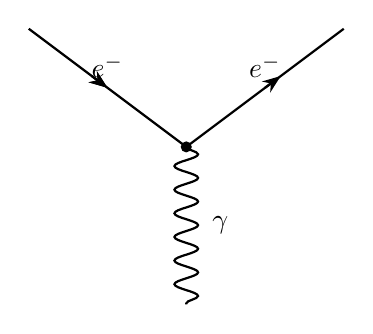
\begin{tikzpicture}[thick, >=Stealth]
\coordinate (v) at (0,0);
\draw[->-] (-2,1.5) -- node[above] {$e^-$} (v);
\draw (v) -- node[above] {$e^-$} (2,1.5);
\draw[decorate, decoration={snake, amplitude=1.5mm, segment length=3mm}] (v) -- node[right=2mm] {$\gamma$} (0,-2);
\fill (v) circle (2pt);
\draw[->] (-1.2,0.9) -- (-1.0,0.75);
\draw[->] (1.0,0.75) -- (1.2,0.9);
\end{tikzpicture}
\end{document}
